\chapter{Introduction}

This report functions as a project plan for an upcoming Master’s thesis to be written in the autumn semester of 2021. The author of the thesis is currently attending the Master’s degree named “Master in Applied Computer Science” and has a prior Bachelor’s degree in Programming (Applications), both attended at NTNU Gjøvik. The thesis will be written in collaboration with the maritime tech startup company called Maritime Optima AS where the author is also employed as a part-time developer.

\section{Topics covered by project}

The shipping industry is an industry where it is still common to use non-digital methods of gathering information and making decisions such as emails, phone calls, and personal expertise. Furthermore, interested parties within the industry rely on predicting the market in order to make favorable decisions and investments. The most important factors impacting the market are cargo demand, and vessel supply (\cref{fig:maritime_economics}). Moreover, since 2004, the International Maritime Organization (IMO) initiated the automated identification system (AIS) protocol and requires all commercial and passenger vessels over 299 gross tonnages (GT) to carry an AIS transponder. This AIS data includes information about the vessel’s position, dimensions, and intended destination making it a prime source for overviewing the current state of a large number of vessels as well as providing a data source for future vessel destination predictions.

\begin{figure}[htbp]  % order of priority: h here, t top, b bottom, p page
    \centering
    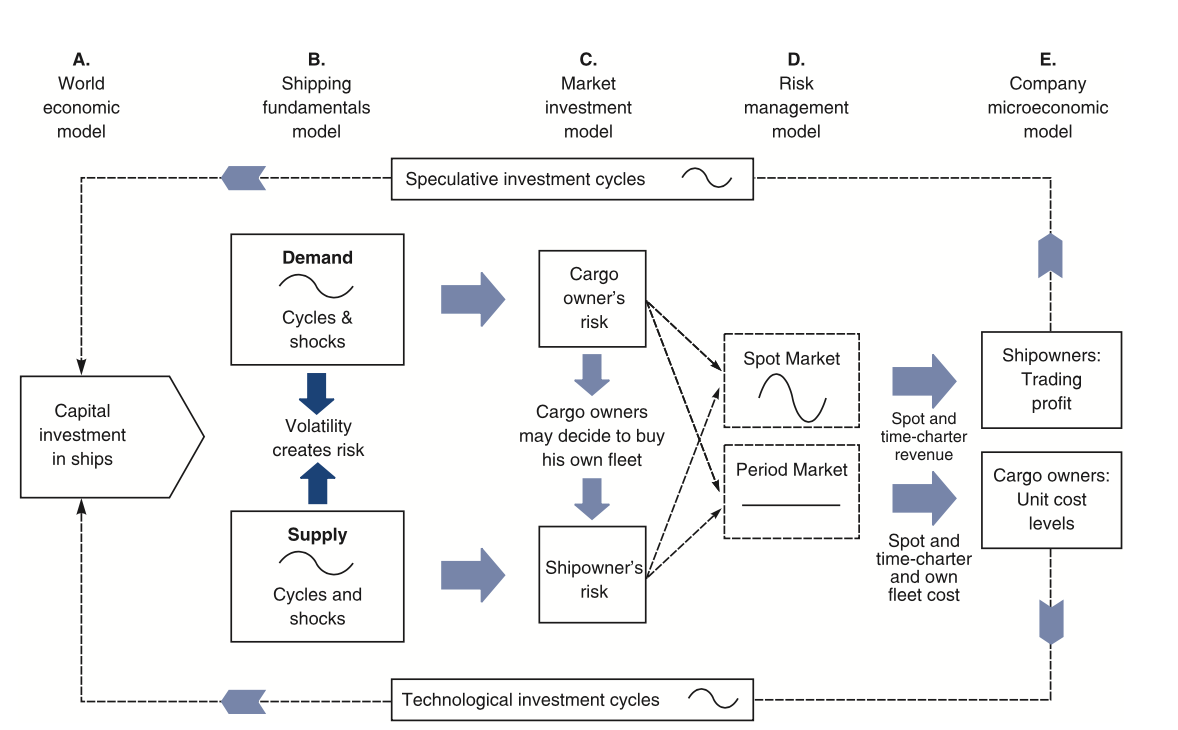
\includegraphics[width=.89\textwidth]{figures/investment_cycle}
    \caption[Map of NTNU Campuses]{Vessel supply’s impact on the market and investment cycles \parencite{stopford2008}}
    \label{fig:maritime_economics}
\end{figure}

The thesis will focus on the research area of maritime vessel destination prediction using established machine learning methods based on historical AIS data. The main purpose of this research is to investigate the possibility of applying prediction methods to a global scale in order to forecast the global vessel supply, or availability, within regions and shipping ports. Applications include supporting ship charterers and operators in their decision-making process and thus improving their ability to optimize their ROI of a portfolio of vessels.

\section{Keywords}

AIS data, vessel destination prediction, supply forecasting, machine learning, maritime logistics

\section{Problem description}

A problem with the current methods used in the shipping industry is that they require manual labor to gather and analyze data. On the other hand, AIS data is plentiful and sufficient for overviewing and forecasting the future state of vessel supply by considering the geographical positions and trajectories of vessels. However, even though the AIS protocol includes attributes for the next destination port and estimated time of arrival (ETA), this information is manually inputted by the crew members of the vessel, and is therefore not standardized and is often exposed to human error either in regards to format or misinformation such as wrong, missing, or outdated information. Therefore, in order to take advantage of AIS data, prediction methods, therefore, only consider geographical information that is automated and accurate. However, since geographical information is considered the best information for vessel predictions, other aspects such as the type and dimensions of the vessel have been overlooked in existing methods limiting them in terms of general accuracy. This thesis will explore the advantages of considering this additional information for vessel destination prediction methods.

\section{Justifications, motivation, and benefits}
\label{section:justifications_motivations_benefits}

The topic of vessel destination prediction using historical AIS data has already been researched as there has been a steady growth of availability of AIS data. There has been a considerable amount of research done into predicting future vessel positions in a short time interval, but little research into using historical AIS data to forecast vessel availability. A paper published at the Hamburg International Conference of Logistics (HICL) in 2019 claims: \textit{“Regarding the forecast of ship-supply so far - to the best of our knowledge - no research has investigated possibilities to predict the number of available ships in a certain region of interest.”} (\cite{lechtenberg2019}) which indicates that this a problem area which has not been explored much. Furthermore, as mentioned in the previous section, the existing methods seem to be lacking in terms of data depth only considering the vessels’ geographical positions and trajectories, while not considering the dimensions and type of the vessels.

\begin{figure}[htbp]  % order of priority: h here, t top, b bottom, p page
    \centering
    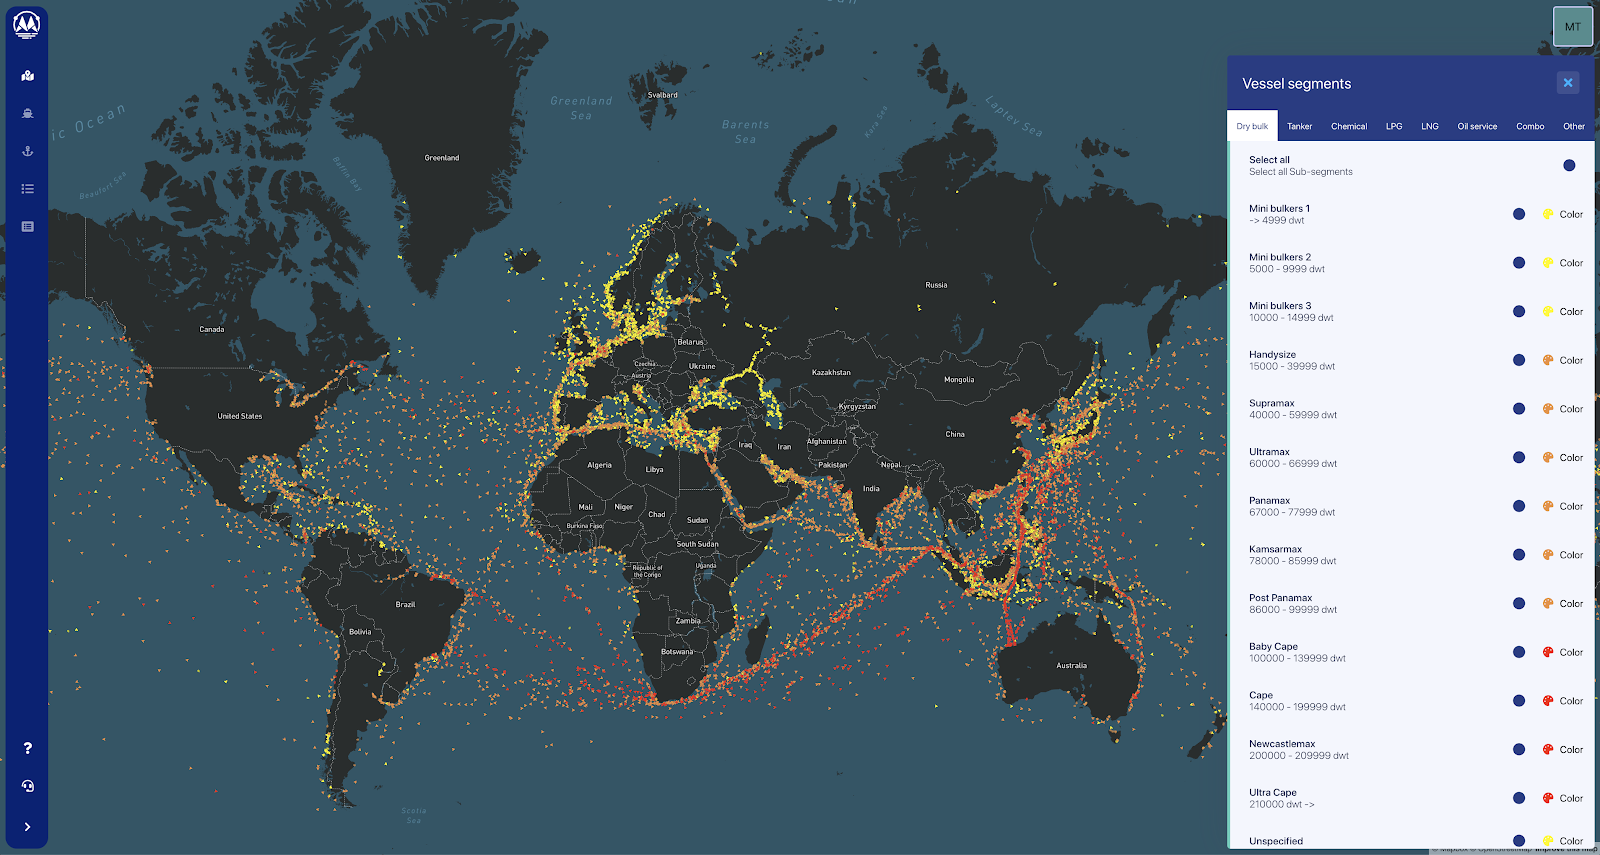
\includegraphics[width=.89\textwidth]{figures/segment_map}
    \caption[Map of NTNU Campuses]{Maritime Optima’s segmentation of vessels where yellow vessels are smaller than reds}
    \label{fig:segment_map}
\end{figure}

The collaborative company Maritime Optima AS has implemented a method of dividing vessels into segments and subsegments (categories and sub-categories). \cref{fig:segment_map} shows the differences in route patterns between different sub-segments (colored from yellow to red relevant to the dimensions of the vessels) for dry cargo vessels. Considering this information in the prediction methods can be a novel approach to the problem area. Maritime Optima has also expressed the novelty of this problem area through thorough competitor analysis and claims that providing accurate predictions is of high value for their customers is a factor that can improve their decision making and investments. Furthermore, the author of the thesis has been employed at Maritime Optima since the founding of the company and has been contributing to the development of their digital platform ever since. These factors combined are the main motivating factors behind this thesis.

\section{Research questions}


\begin{enumerate}
    \item What prediction methods can be used to predict vessel availability?
    \item What prediction methods can be used to predict vessel destinations?
    \begin{enumerate}
        \item What type of data did they rely on?
        \item How much depth of the data was relevant to the results?
        \item How successful were they at predicting vessel destinations?
        \item How applicable were they toward predicting vessel availability?
    \end{enumerate}
    \item How can the quality of the prediction methods be ensured?
    \begin{enumerate}
        \item What metrics, or measurements, are used to establish quality?
    \end{enumerate}
    \item How extensive is the impact of considering segmentation for prediction methods?
\end{enumerate}

\section{Planned contributions}

The main contribution of the thesis will consist of extending and improving existing prediction models by increasing the depth of the data with Maritime Optima’s novel segmentation of vessels. Considering the time limitations of the thesis, this is the most important aspect to explore in the thesis. The second contribution of the thesis will include extending the scale of the prediction methods by applying it to Maritime Optima’s global set of vessels in order to forecast availability, and supply, for regions and ports. Both areas are little-explored topics and this will, therefore, contribute to the state of the art of the existing literature.


Another important goal of the research is also to establish a foundation that can easily be further improved upon by continuing to add more data attributes from either the AIS protocol or external sources such as Maritime Optima’s extensive vessel database, or user-supplied information.
